\chapter{Binary Search Trees}
\label{ch:bst}

\newcommand{\lecnum}{15}
%\newcommand{\lectitle}{Binary Search Trees}
\newcommand{\lecturer}{Frank Pfenning, Andr\'e Platzer, Rob Simmons,
  Iliano Cervesato}

\chapterTAGS{bst, complexity, correctness, dictionary, divide-and-conquer, ds-invariant, function-pointer, interface, ordering, safety, search, set}
\maketitle

\begin{preamble}
\noindent
In this lecture, we will continue considering ways to implement the
dictionary (or associative array) interface.  This time, we will implement
this interface with \emph{binary search trees}.  We will eventually be
able to achieve $O(\log n)$ worst-case asymptotic complexity for
insert and lookup.  This also extends to delete, although we won't
discuss that operation in lecture.

%% This means that while hash tables (with appropriate amounts of
%% resizing and rehashing) have a better average-case performance than
%% binary search trees, binary search trees

%% \emph{worst-case} complexity of associative array operations
%% implemented as binary search trees is better than the worst-case
%% complexity when implemented as hash tables, because we were only able
%% to get reasonable \emph{average-case}
\end{preamble}

\begin{gram}[Learning Goals]
This fits as follows with respect to our learning goals:
\begin{description}
\item[Computational Thinking: ]%
  We discover binary trees as a way to organize information.  We superimpose
  to them the notion of sortedness, which we examined in the past, as a way to
  obtain exponential speedups.

\item[Algorithms and Data Structures: ]%
  We present binary search trees as a space-efficient and extensible data
  structure with a potentially logarithmic complexity for many operations of
  interest --- we will see in the next lecture how to guarantee this bound.

\item[Programming: ]%
  We define a type for binary trees and use recursion as a convenient approach
  to implement specification functions and operations on them.
\end{description}
\end{gram}


\section{Ordered Collections}
\label{ch:bst:intro_ordered}
\TAGS{ordering}

Hash dictionaries organize entries in an array at indices that are
determined from their key using a hash function.  If the hash function
is good, this means that the entries will be placed at a reasonably
random position spread out across the whole array. If it is bad,
linear search is needed to locate the entry.

There are many alternative ways of implementing dictionaries.  For
example, we could have stored the entries in an array, sorted by key.
Then lookup by binary search would have been $O(\log n)$, but
insertion would be $O(n)$, because it takes $O(\log n)$ steps to find
the right place, but then $O(n)$ steps to make room for that new entry
by shifting all elements with a bigger key over.  (We would also need
to grow the array as in unbounded arrays to make sure it does not run
out of capacity.)  Arrays are not flexible enough for fast insertion,
but the data structure that we will be devising in this lecture will
be.


\section{Abstract Binary Search}
\label{sec:bst:abstracting_binsearch}
\TAGS{divide-and-conquer, ordering}

What are the operations that we needed to be able to perform binary
search?  We needed a way of comparing the key we were looking for with
the key of a given entry in our data structure.  Depending on the
result of that comparison, binary search returns the position of that
entry if they were the same, advances to the left if what we are
looking for is smaller, or advances to the right if what we are
looking for is bigger.  For binary search to work with the complexity
$O(\log n)$, it was important that binary search advances to the left
or right \emph{many steps at once}, not just by one element.  Indeed,
if we would follow the abstract binary search principle starting from
the middle of the array but advancing only by one index in the array,
we would obtain linear search, which has complexity $O(n)$, not
$O(\log n)$.

Thus, binary search needs a way of comparing keys and a way of
advancing through the elements of the data structure very quickly,
either to the left (towards entries with smaller keys) or to the
right (towards bigger ones).  In the array-based binary search we've
studied, each iteration calculates a midpoint
\begin{lstlisting}[language={[C0]C}]
   int mid = lo + (hi - lo) / 2;
\end{lstlisting}
and a new bound for the next iteration is (if the key we're searching
for is smaller than that of the entry at \lstinline'mid')
\begin{lstlisting}[language={[C0]C}]
   hi = mid;
\end{lstlisting}
or (if the key is larger)
\begin{lstlisting}[language={[C0]C}]
   lo = mid + 1;
\end{lstlisting}
Therefore, we know that the next value \lstinline'mid' will be either
\lstinline'(lo + mid) / 2' or
\lstinline'((mid + 1) + hi) / 2'
(ignoring the possibility of overflow).

This pattern continues, and given any sorted array, we can enumerate
all possible binary searches:
\begin{center}
  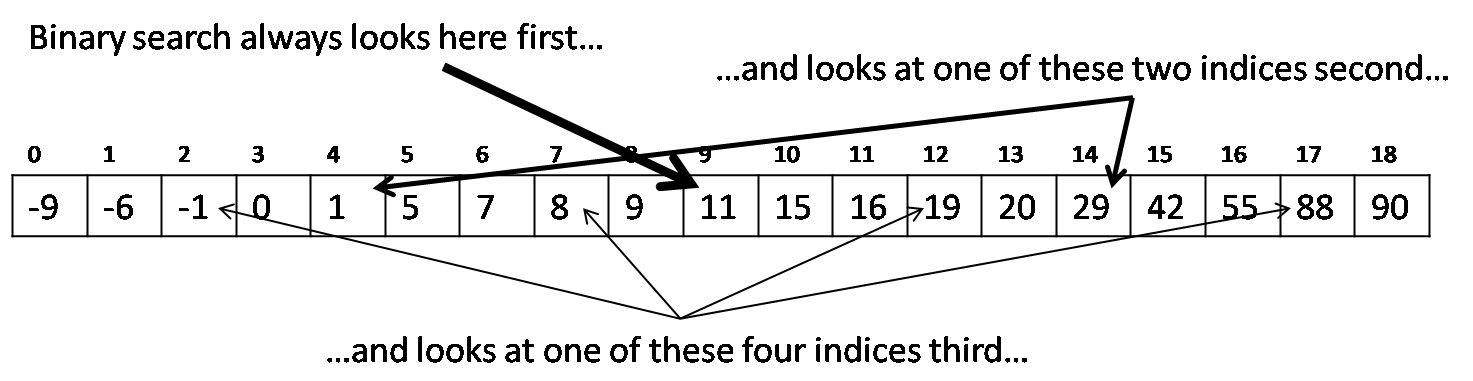
\includegraphics[width=0.95\textwidth]{img/abstract-bst1.png}
\end{center}

This pattern means that constant-time access to an array element at an
\emph{arbitrary} index isn't necessary for doing binary search! To do
binary search on the array above, all we need is constant time access
from array index 9 (containing 11) to array indices 4 and 14
(containing 1 and 29, respectively), constant time access from array
index 4 to array indices 2 and 7, and so on. At each point in binary
search, we know that our search will proceed in one of at most two
ways, so we will explicitly represent those choices with a pointer
structure, giving us the structure of a \emph{binary tree}. The tree
structure that we got from running binary search on this array\ldots
\begin{center}
  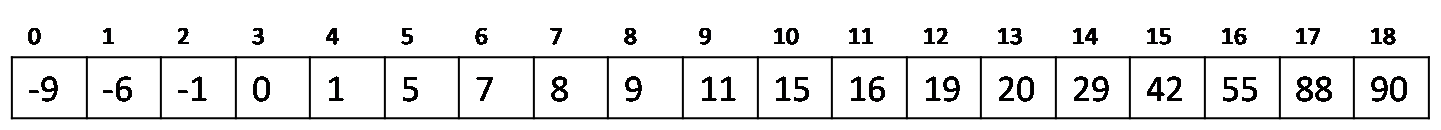
\includegraphics[width=0.95\textwidth]{img/abstract-bst2.png}
\end{center}
\ldots corresponds to this binary tree:
\begin{center}
  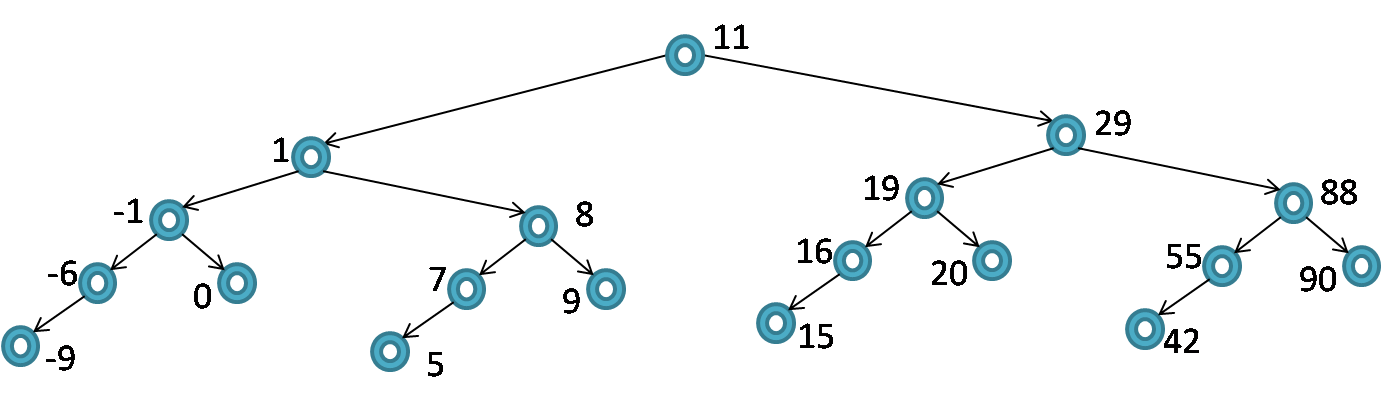
\includegraphics[width=0.95\textwidth]{img/abstract-bst3.png}
\end{center}

%% arrays give us


%% In Lecture 6, we
%% also saw that both computations might actually overflow in arithmetic,
%% so we devised a more clever way of computing the midpoint, but we will
%% ignore this for simplicity here.  In Lecture 6, we also did consider
%% \lstinline'int' as the data type. Now we study data of an arbitrary type
%% \lstinline'entry' provided by the client.  In particular, as one step of
%% abstraction, we will now actually compare entries in terms of their
%% keys.

%% Unfortunately, inserting into arrays remains an $O(n)$ operation.
%% For other data structures, insertion is easy. For example, insertion into a doubly linked list at a given list node is $O(1)$.
%% But if we use a sorted doubly linked list, the insertion step will be easy, but finding the right position by binary search is challenging, because we can only advance one step to the left or right in a doubly linked list.
%% That would throw us back into linear search through the list to find the entry, which gives a lookup complexity of $O(n)$.
%% How can we combine the advantages of both:
%% fast navigation by several elements as in arrays, together with fast insertion as in doubly linked lists?
%% % Before you read on, try to see if you can find an answer yourself.

%% In order to obtain the advantages of both, and, thus, enable binary search on a data structure that supports fast insertion, we proceed as follows.
%% The crucial observation is that arrays provide fast access to any arbitrary index in the array, which is why they are called a random access data structure, but binary search only needs very selective access from each entry.
%% Whatever key binary search is looking at, it only needs access to that entry and one (sufficiently far away) left entry and one (sufficiently far away) right entry.
%% If binary search has just looked at index \lstinline'mid', then it will subsequently only look at either \lstinline'(lo + mid) / 2' or \lstinline'(mid+1 + hi) / 2'.
%% In particular, for each entry, we need to remember what its key is, what its left successor is and what its right successor is, but nothing else.
%% We use this insight to generalize the principle behind binary search to a more general data structure.


\section{Representing Binary Trees with Pointers}
\label{sec:bst:tree_structure}
\TAGS{bst, ds-invariant, function-pointer, ordering}

%Unlike heaps, we cannot easily represent binary search trees with
%arrays and keep them balanced in the way we preserved the heap
%invariant. This is because with heaps where was a lot of flexibility
%where to insert new entries, while with binary search trees the
%position of the new entry seems rather rigidly
%determined\footnote{although we will see next lecture that this is not
%  strictly true}. So
To represent a binary tree using pointers, we use a struct with
two pointers: one to the left child and one to the
right child.  If there is no child, the pointer is \lstinline'NULL'. A leaf
of the tree is a node with two \lstinline'NULL' pointers.

\begin{lstlisting}[language={[C0]C}]
typedef struct tree_node tree;
struct tree_node {
  entry data;       // Non NULL
  tree* left;
  tree* right;
};
\end{lstlisting}
Rather than the fully generic data implementation that we used for
hash tables, we'll assume for the sake of simplicity that the client
is providing us with two types, a pointer type \lstinline'entry'
corresponding to entries and a type \lstinline'key' for their keys,
and with two functions, \lstinline'entry_key' that returns the key of
an entry and \lstinline'key_compare' that compares two keys:

\begin{lstlisting}[language={[C0]C}]
/* Client-side interface */
// typedef ______  key;
// typedef ______* entry;

key entry_key(entry e)
/*@requires e != NULL; @*/ ;

int key_compare(key k1, key k2)
/*@ensures -1 <= \result && \result <= 1; @*/ ;
\end{lstlisting}
We require that valid values of type \lstinline'entry' be
non-\lstinline'NULL'.  As usual, our implementation of dictionaries
based on trees will use \lstinline'NULL' to signal that an
\lstinline'entry' is not there.

The function \lstinline'key_compare' provided by the client is different
from the equivalence function we used for hash tables.  For binary
search trees, we need to compare keys $k_1$ and $k_2$ and
determine if $k_1 < k_2$, or $k_1 = k_2$, or $k_1 > k_2$.  A common
approach to this is for a comparison function to return an integer
$r$, where $r < 0$ means $k_1 < k_2$, $r = 0$ means $k_1 = k_2$, and
$r > 0$ means $k_1 > k_2$.  Our contract captures that we expect
\lstinline'key_compare' to return no values other than -1, 0, and 1.

Trees are the second \emph{recursive} data structure we've seen: a tree
node has two fields that contain pointers to tree nodes. Thus far
we've only seen recursive data structures as linked lists, either
chains in a hash table or list segments in a stack or a queue.

Let's remember how we picture list segments. Any list segment is referred to
by two pointers, \lstinline'start' and \lstinline'end', and there are two
possibilities for how this list can be constructed, both of which require
\lstinline'start' to be non-\lstinline'NULL' (and \lstinline'start->data' also
to satisfy our constraints on \lstinline'entry' values).
\begin{lstlisting}[language={[C0]C}]
bool is_segment(list* start, list* end) {
  if (start == NULL) return false;
  if (start->data == NULL) return false;
  if (start == end) return true;
  return is_segment(start->next, end);
}
\end{lstlisting}
We can represent these choices graphically by using a picture like

\includegraphics[width=0.04\textwidth]{img/segment-pic.png}
to represent an arbitrary segment. Then we know every segment has one or two
forms:
\begin{center}
  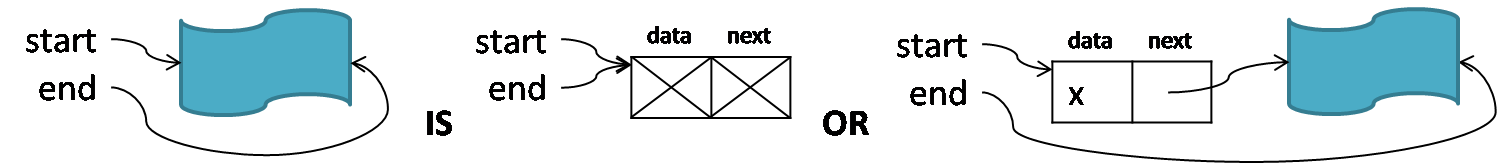
\includegraphics[width=0.9\textwidth]{img/segment-cases.png}
\end{center}

We'll create a similar picture for trees: the tree containing no
entries is \lstinline'NULL', and a non-empty tree is a struct with three
fields: the data and the \lstinline'left' and \lstinline'right' pointers, which
are themselves trees.
\begin{center}
  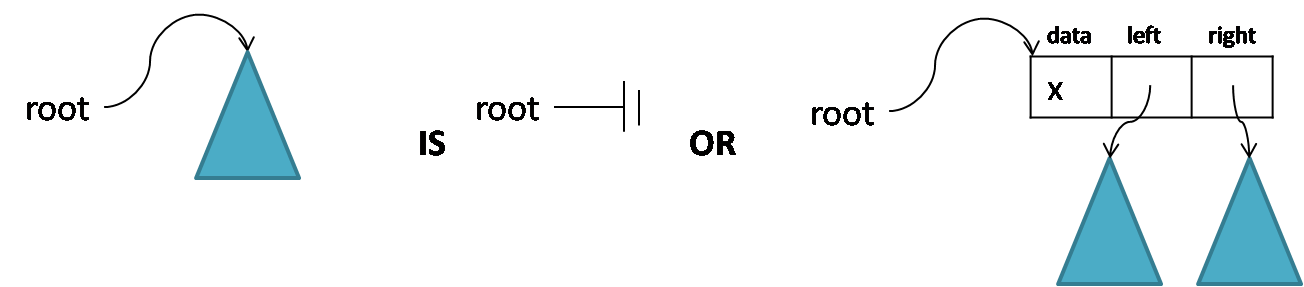
\includegraphics[width=0.9\textwidth]{img/bst-cases.png}
\end{center}
Rather than drawing out the \lstinline'tree_node' struct with its three
fields explicitly, we'll usually use a more graph-like way of
presenting trees:
\begin{center}
  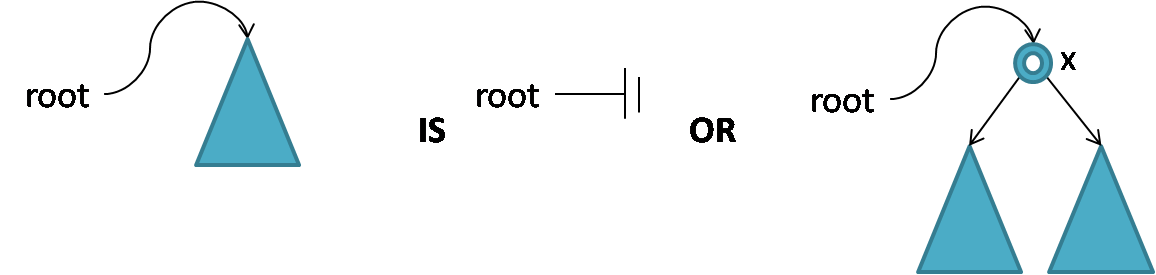
\includegraphics[width=0.9\textwidth]{img/bst-cases2.png}
\end{center}

This recursive definition can be directly encoded into a very simple
data structure invariant \lstinline'is_tree'. It checks very little: just
that all the \lstinline'data' fields are non-\lstinline'NULL', as the client
interface requires. If it terminates, it also ensures that there are no cycles;
a cycle would cause non-termination, just as it would with
\lstinline'is_segment'.
\begin{lstlisting}[language={[C0]C}]
bool is_tree(tree* root) {
  if (root == NULL) return true;
  return root->data != NULL
      && is_tree(root->left) && is_tree(root->right);
}
\end{lstlisting}


\subsection{The Ordering Invariant}

Binary search was only correct for arrays if the array was sorted.
Only then do we know that it is okay not to look at the upper half of
the array if the element we are looking for is smaller than the middle
element, because, in a sorted array, it can then only occur in the
lower half, if at all.  For binary search to work correctly on binary
search trees, we, thus, need to maintain a corresponding data
structure invariant: all entries to the right of a node have keys
that are bigger than the key of that node.  And all the nodes to the
left of that node have smaller keys than the key at that node.  This
\emph{ordering invariant} is a core idea of binary search trees; it's
what makes a binary tree into a binary \emph{search} tree.

\begin{quote}
  \noindent\textbf{Ordering Invariant.} At any node with key $k$ in a
  binary search tree, the key of all entries in the left subtree is
  strictly less than $k$, while the key of all entries in the right
  subtree is strictly greater than $k$.
\end{quote}
This invariant implies that no key occurs more than once in a tree,
and we have to make sure our insertion function maintains this
invariant.

We won't write code for checking the ordering invariant just yet, as
that turns out to be surprisingly difficult. We'll first discuss the
lookup and insertion functions for binary search trees.  As we carry
out this discussion, we will assume we have a function
\lstinline'is_bst(T)' that incorporates \lstinline'is_tree' seen
earlier and the ordering invariant.  We will implement
\lstinline'is_bst' later in this lecture.

%% \section{Binary Search in Binary Search Trees}
%% The data structure we have developed so far results in a (binary)
%% tree.  A binary tree consists of a set of nodes and, for each node,
%% its left and its right child.  Finding an entry in a binary search
%% tree follows exactly the same idea that binary search did, just on a
%% more abstract data structure:
%% What do we need to know about the binary tree to make sure that this principle will always lookup entries correctly?
%% What data structure invariant do we need to maintain for the binary search tree?

\section{Searching for a Key}
\label{sec:bst:searching}
\TAGS{bst, dictionary, search}

The ordering invariant lets us find an entry with key $k$ in a
binary search tree the same way we found an entry with binary
search, just on the more abstract tree data structure.  Here is a
recursive algorithm for search, starting at the root of the tree:

\begin{enumerate}
\item If the tree is empty, stop.
\item Compare the key $k'$ of the current node to $k$. Stop if equal.
\item If $k$ is smaller than $k'$, proceed to the left child.
\item If $k$ is larger than $k'$, proceed to the right child.
\end{enumerate}
The implementation of this search captures the informal description
above.  Recall that \lstinline'entry_key(e)' extracts the key component
of entry \lstinline'e' and that \lstinline'key_compare(k1,k2)'
returns \lstinline'-1' if $k_1 < k_2$, \lstinline'0' if $k_1 = k_2$,
and \lstinline'1' if $k_1 > k_2$.
\begin{lstlisting}[language={[C0]C}]
entry bst_lookup(tree* T, key k)
/*@requires is_bst(T); @*/
/*@ensures \result == NULL
        || key_compare(entry_key(\result), k) == 0; @*/
{
  if (T == NULL) return NULL;

  int cmp = key_compare(k, entry_key(T->data));
  if (cmp == 0)  return T->data;
  if (cmp <  0)  return bst_lookup(T->left, k);
  //@assert cmp > 0;
  return bst_lookup(T->right, k);
}
\end{lstlisting}
We chose here a recursive implementation, following the structure of a
tree, but in practice an iterative version may also be a reasonable
alternative (see Exercise~\ref{ex:bst_lookup-iterative}).  We also chose
to return not a Boolean but either the entry itself if it matches
the key \lstinline'k' given in input, and \lstinline'NULL' otherwise.
In this way, we can use our burgeoning binary search tree support both
to implement dictionaries and sets --- for a set, the types
\lstinline'key' and \lstinline'entry' are the same and the function
\lstinline'entry_key' simply returns its argument.


\section{Complexity}
\label{sec:bst:complexity}
\TAGS{bst, complexity}

If our binary search tree were perfectly balanced, that is, had the
same number of nodes on the left as on the right for every subtree,
then the ordering invariant would ensure that search for an entry
with a given key has asymptotic complexity $O(\log n)$, where $n$ is
the number of entries in the tree. Every time we compare the key
\lstinline'k' with the root of a perfectly balanced tree, we either
stop or throw out half the entries in the tree.

In general we can say that the cost of lookup is $O(h)$, where $h$ is
the \emph{height} of the tree. We will define height to be the maximum
number of nodes that can be reached by any sequence of pointers
starting at the root. An empty tree has height 0, and a tree with two
children has the maximum height of either child, plus 1.

%% Why? When searching for a
%% given key $k$ in the tree, we just compare $k$ with the key $k'$ of
%% the entry at the root. If they are equal, we have found the entry. If
%% $k < k'$ we recursively search in the left subtree, and if $k' < k$ we
%% recursively search in the right subtree. This is just like binary
%% search, except that instead of an array we traverse a tree data
%% structure.
%% Unlike in an array, however, we will see that insertion is quick as well.


\section{The Interface}
\label{sec:bst:interface}
\TAGS{bst, interface}

Before we talk about insertion into a binary search tree, we should
recall the interface of dictionaries and discuss how we will implement
it.  Remember that we're assuming a client definition of types
\lstinline'entry' and \lstinline'key', and functions
\lstinline'entry_key' and \lstinline'key_compare', rather than the
fully generic version using void pointers and function pointers.

\begin{lstlisting}[language={[C0]C}]
/* Library interface */
// typedef ______* dict_t;

dict_t dict_new()
/*@ensures \result != NULL; @*/ ;

entry dict_lookup(dict_t D, key k)
/*@requires D != NULL; @*/
/*@ensures \result == NULL
        || key_compare(entry_key(\result), k) == 0; @*/ ;

void dict_insert(dict_t D, entry e)
/*@requires D != NULL && e != NULL; @*/
/*@ensures dict_lookup(D, entry_key(e)) != NULL; @*/ ;
\end{lstlisting}

We can't define the type \lstinline'dict_t' to be \lstinline'tree*',
for two reasons.  One reason is that a new tree should be empty, but
an empty tree is represented by the pointer \lstinline'NULL', which
would violate the \lstinline'dict_new' postcondition.  More
fundamentally, if \lstinline'NULL' was the representation of an empty
dictionary, there would be no way to write a function to imperatively
insert additional entries.  This is because a function call makes
copies of the (small) values passed as arguments.

The usual solution here is one we have already used for stacks,
queues, and hash tables: we have a \emph{header} which in this case
just consists of a pointer to the root of the tree.  We often keep
other information associated with the data structure in these headers,
such as the size.

\begin{lstlisting}[language={[C0]C}]
struct dict_header {
  tree* root;
};
typedef struct dict_header dict;

bool is_dict(dict* D) {
  return D != NULL && is_bst(D->root);
}
\end{lstlisting}
Lookup in a dictionary then just calls the recursive function
we've already defined:
\begin{lstlisting}[language={[C0]C}]
entry dict_lookup(dict* D, key k)
/*@requires is_dict(D); @*/
/*@ensures \result == NULL
        || key_compare(entry_key(\result), k) == 0; @*/
{
  return bst_lookup(D->root, k);
}
\end{lstlisting}
The relationship between the functions \lstinline'is_dict' and
\lstinline'is_bst' and between \lstinline'dict_lookup' and
\lstinline'bst_lookup' is a common one. The non-recursive function
\lstinline'is_dict' is given the non-recursive struct
\lstinline'dict_header', and then calls the recursive helper function
\lstinline'is_bst' on the recursive structure of tree nodes.


\section{Inserting an Entry}
\label{sec:bst:insertion}
\TAGS{bst, correctness, dictionary, ds-invariant, safety}

With the header structure, it is straightforward to implement
\lstinline'bst_insert'.  We just proceed as if we were looking for the
given entry. If we find a node with the same key, we just overwrite
its \lstinline'data' field.  Otherwise, we insert the new entry in
the place where it would have been, had it been there in the first
place.  This last clause, however, creates a small difficulty.  When
we hit a null pointer (which indicates the key was not already in the
tree), we cannot replace what it points to (it doesn't point to
anything!).  Instead, we \emph{return} the new tree so that the parent
can modify itself.

\newpage
\begin{lstlisting}[language={[C0]C}]
tree* bst_insert(tree* T, entry e)
/*@requires is_bst(T) && e != NULL; @*/
/*@ensures is_bst(\result)
        && bst_lookup(\result, entry_key(e)) != NULL; @*/
{
  if (T == NULL) {
    /* create new node and return it */
    tree* R  = alloc(tree);
    R->data  = e;
    R->left  = NULL;  // Not required (initialized to NULL)
    R->right = NULL;  // Not required (initialized to NULL)
    return R;
  }

  int cmp = key_compare(entry_key(e), entry_key(T->data));
  if (cmp == 0)     T->data = e;
  else if (cmp < 0) T->left = bst_insert(T->left, e);
  else {
    //@assert cmp > 0;
    T->right = bst_insert(T->right, e);
  }
  return T;
}
\end{lstlisting}

The returned subtree will
also be stored as the new root:

\begin{lstlisting}[language={[C0]C}]
void dict_insert(dict* D, entry e)
//@requires is_dict(D) && e != NULL;
/*@ensures  is_dict(D)
        && dict_lookup(D, entry_key(e)) != NULL; @*/
{
  D->root = bst_insert(D->root, e);
}
\end{lstlisting}

\section{Checking the Ordering Invariant}
\label{sec:bst:bst_invariant}
\TAGS{ds-invariant, ordering}

When we analyze the structure of the recursive functions implementing
search and insert, we are tempted to try defining a simple,
\emph{but wrong!} ordering invariant for binary trees as follows:
tree $T$ is ordered whenever
\begin{enumerate}
\item $T$ is empty, or
\item $T$ has key $k$ at the root, $T_L$ as left subtree and $T_R$ as
  right subtree, and
  \begin{itemize}
  \item $T_L$ is empty, or $T_L$'s key is less than $k$ and $T_L$ is
    ordered; and
  \item $T_R$ is empty, or $T_R$'s key is greater than $k$ and $T_R$
    is ordered.
  \end{itemize}
\end{enumerate}
This would yield the following code:
\begin{lstlisting}[language={[C0]C}]
/* THIS CODE IS BUGGY */
bool is_ordered(tree* T) {
  if (T == NULL) return true;  /* an empty tree is a BST */
  key k = entry_key(T->data);
  return (T->left == NULL
          || key_compare(entry_key(T->left->data), k) < 0)
      && (T->right == NULL
          || key_compare(k, entry_key(T->right->data)) < 0)
      && is_ordered(T->left)
      && is_ordered(T->right);
}
\end{lstlisting}
While this should always be true for a binary search tree, it is far
weaker than the ordering invariant stated at the beginning of lecture.
Before reading on, you should check your understanding of that
invariant to exhibit a tree that would satisfy the above code, but
violate the ordering invariant.

\clearpage
There is actually more than one problem with this.  The most
glaring one is that following tree would pass this test:
\begin{center}
  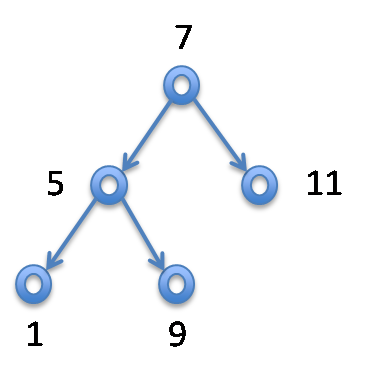
\includegraphics[width=0.3\textwidth]{img/bst1.png}
\end{center}
Even though, locally, the key of the left node is always
smaller and on the right is always bigger, the node with
key $9$ is in the wrong place and we would not find it
with our search algorithm since we would look in the right
subtree of the root.

An alternative way of thinking about the invariant is as follows.
Assume we are at a node with key $k$.
\begin{enumerate}
\item If we go to the \emph{left} subtree, we establish an
\emph{upper bound} on the keys in the subtree: they must
all be smaller than $k$.
\item If we go to the \emph{right} subtree, we establish a
\emph{lower bound} on the keys in the subtree: they must
all be larger than $k$.
\end{enumerate}
The general idea then is to traverse the tree recursively, and pass
down an interval with lower and upper bounds for all the keys in the
tree.  The following diagram illustrates this idea on a tree with
integer entries.  We start at the
root with an unrestricted interval, allowing any key, which is written
as $(-\infty, +\infty)$.  As usual in mathematics we write intervals
as $(x,z) = \{y \mid x < y\;\mbox{and}\; y < z\}$.  At the leaves we
write the interval for the subtree.  For example, if there were a
left subtree of the node with key $7$, all of its keys would have
to be in the interval $(5,7)$.
\begin{center}
  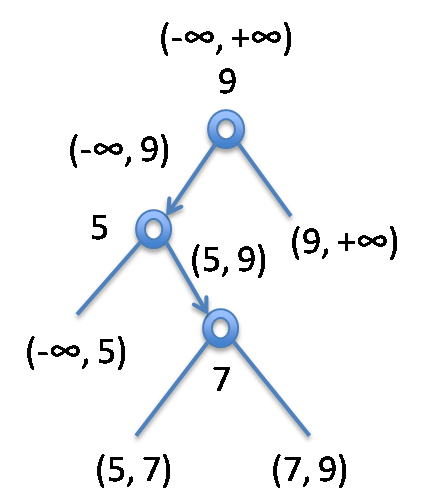
\includegraphics[width=0.35\textwidth]{img/bst4.png}
\end{center}

The only difficulty in implementing this idea is the unbounded
intervals, written above as $-\infty$ and $+\infty$.  Here is one
possibility: we pass not just the key value, but the particular entry
from which we can extract the key that bounds the tree. Since
\lstinline'entry' must be a pointer type,
this allows us to pass \lstinline'NULL' in case there is no lower or upper
bound.
\begin{lstlisting}[language={[C0]C}]
bool is_ordered(tree* T, entry lo, entry hi)
//@requires is_tree(T);
{
  if (T == NULL) return true;
  key k = entry_key(T->data);
  return T->data != NULL
      && (lo == NULL || key_compare(entry_key(lo), k) < 0)
      && (hi == NULL || key_compare(k, entry_key(hi)) < 0)
      && is_ordered(T->left, lo, T->data)
      && is_ordered(T->right, T->data, hi);
}
\end{lstlisting}

We can then combine our earlier (and admittedly minimal)
\lstinline'is_tree' and \lstinline'is_ordered' into a function that
checks whether a given tree is a binary search tree, and using it we
can define a representation invariant function for dictionaries
implemented as binary search trees:

\begin{lstlisting}[language={[C0]C}]
bool is_bst(tree* T) {
  return is_tree(T) && is_ordered(T, NULL, NULL);
}

bool is_dict(dict* D) {
  return D != NULL && is_bst(D->root);
}
\end{lstlisting}

A word of caution: the call to \lstinline'is_ordered(T, NULL, NULL)'
embedded in the pre- and
post-condition of the function \lstinline'bst_insert' is actually not
strong enough to prove the correctness of the recursive function.  A
similar remark applies to \lstinline'bst_lookup'.  This is because of
the missing information of the bounds.  We will return to this issue
later in the course.


\section{BST Sets}
\label{sec:bst:sets}
\TAGS{bst, interface, set}

As we saw when talking about hash tables, a set is a dictionary whose
keys and entries are the same thing --- they are the elements of the
set.  Therefore, just like with hash tables, we can base an
implementation of sets on binary search trees.  The interface a BST
set library is as follows:

\begin{lstlisting}[language={[C0]C}]
/* Client-side interface */
// typedef ______  elem;

int elem_compare(elem e1, elem e2)
/*@ensures -1 <= \result && \result <= 1; @*/ ;


/* Library interface */
// typedef ______* set_t;

set_t set_new()
/*@ensures \result != NULL; @*/ ;

bool set_contains(set_t S, elem e)
/*@requires S != NULL; @*/ ;

void set_insert(set_t S, elem e)
/*@requires S != NULL; @*/
/*@ensures S != NULL && set_contains(S, e) != NULL; @*/ ;
\end{lstlisting}

Because lookup (now a set membership test) returns a boolean, there is
no reason for elements to be pointers.


\section{The Shape of Binary Search Trees}
\label{sec:bst:shape}
\TAGS{bst, complexity}

We have already mentioned that balanced binary search trees have good
properties, such as logarithmic time for insertion and search.
The question is if binary search trees will be balanced.  This
depends on the order of insertion.  Consider the insertion of
numbers $1$, $2$, $3$, and $4$.

If we insert them in increasing order we obtain the following trees
in sequence.
\begin{center}
  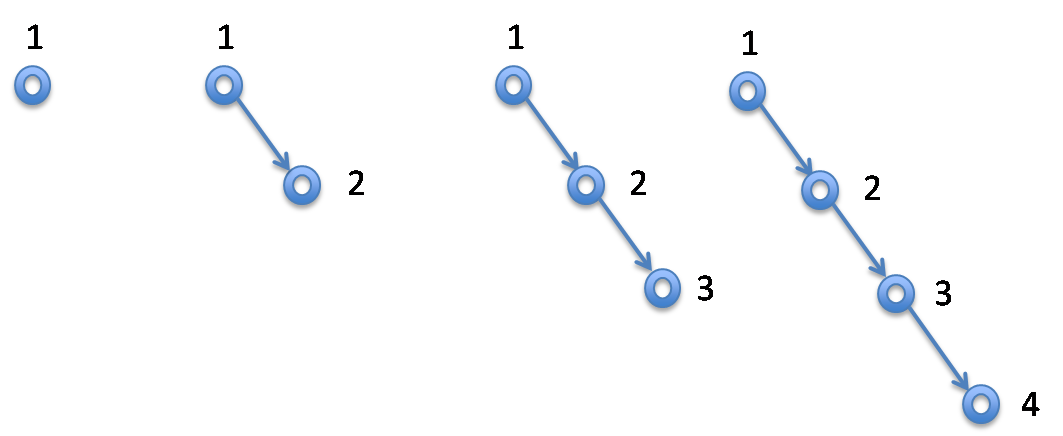
\includegraphics[width=0.7\textwidth]{img/bst2.png}
\end{center}
Similarly, if we insert them in decreasing order we get a straight
line, always going to the left.  If we instead insert in
the order 3, 1, 4, 2, we obtain the following sequence of binary
search trees:
\begin{center}
  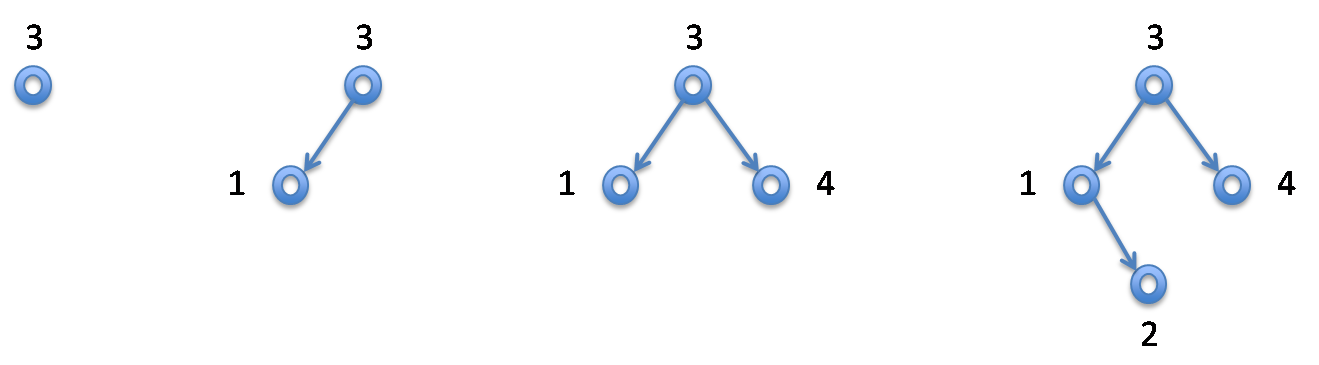
\includegraphics[width=0.9\textwidth]{img/bst3.png}
\end{center}
Clearly, the last tree is much more balanced.  In the extreme, if
we insert entries with their keys in order, or reverse order, the
tree will be linear, and search time will be $O(n)$
for $n$ items.

These observations mean that it is extremely important to pay
attention to the balance of the tree.  We will discuss ways
to keep binary search trees balanced in the next lecture.

\clearpage
\section{Exercises}
\label{sec:bst:exercises}

\begin{flex}
\begin{exercise}%[\opt{sample solution on page~\pageref{ex:bst-insert-24-33-10-2-1-7-6-solved}}]
\label{ex:bst-insert-24-33-10-2-1-7-6}
  Draw the binary search tree resulting from inserting the following
  numbers in the given order starting from an empty tree.
  \begin{center}
    24, \ \ \ 33, \ \ \ 10, \ \ \ 2, \ \ \ 1, \ \ \ 7, \ \ \ 6
  \end{center}
\end{exercise}

\begin{solution}\opt{\textbf{of exercise~\ref{ex:bst-insert-24-33-10-2-1-7-6}}}
\label{ex:bst-insert-24-33-10-2-1-7-6-solved}
\begin{center}
  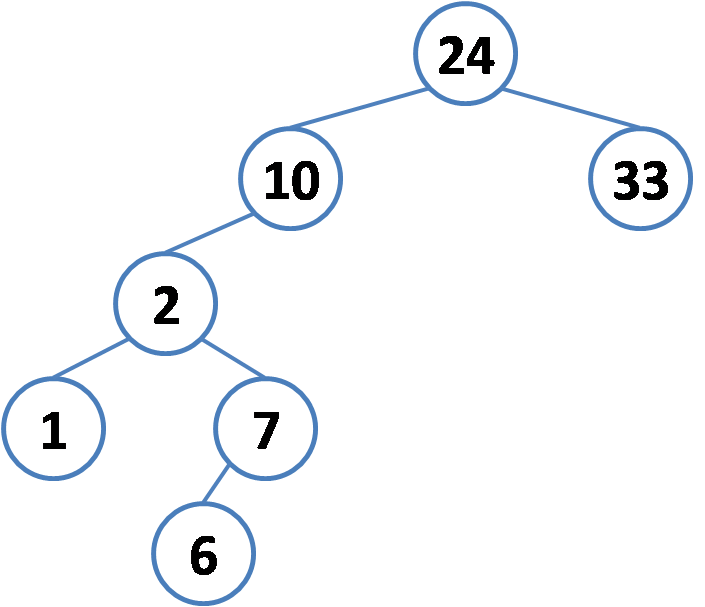
\includegraphics[width=0.5\textwidth]{img/bst-ex1.png}
\end{center}
\end{solution}
\end{flex}


\begin{flex}
\begin{exercise}%[\opt{sample solution on page~\pageref{ex:bst_lookup-iterative-solved}}]
  %[Iterative Lookup]
\label{ex:bst_lookup-iterative}
  Rewrite \lstinline'dict_lookup' to be iterative rather than rely on
  the recursive helper function \lstinline'bst_lookup'.
\end{exercise}

\begin{solution}\opt{\textbf{of exercise~\ref{ex:bst_lookup-iterative}}}
\label{ex:bst_lookup-iterative-solved}
\begin{lstlisting}[language={[C0]C}]
entry dict_lookup(dict* D, key k)
/*@requires is_dict(D); @*/
/*@ensures \result == NULL
        || key_compare(entry_key(\result), k) == 0; @*/
{
  tree* T = D->root;
  while (T != NULL) {
    int cmp = key_compare(k, entry_key(T->data));
    if (cmp = 0) return T->data;
    if (cmp < 0) T = T->left;
    else { //@assert cmp > 0;
      T = T->right;
    }
  }
  //@assert T == NULL;
  return NULL;
}
\end{lstlisting}
\end{solution}
\end{flex}


\begin{flex}
\begin{exercise}%[\opt{sample solution on page~\pageref{ex:bst_insert-iterative-solved}}]
\label{ex:bst_insert-iterative}
  Rewrite \lstinline'bst_insert' to be iterative rather than rely on
  the recursive helper function \lstinline'bst_insert'.
  [\noindent\textbf{Hint:} The difficulty will be to update the
  pointers in the parents when we replace a node that is
  \lstinline'NULL'.  For that purpose we can keep a ``trailing''
  pointer which should be the parent of the node currently under
  consideration.]
\end{exercise}

\begin{solution}\opt{\textbf{of exercise~\ref{ex:bst_insert-iterative}}}
\label{ex:bst_insert-iterative-solved}
\begin{lstlisting}[language={[C0]C}]
void dict_insert(dict* D, entry e)
/*@requires is_dict(D) && e != NULL; @*/
/*@ensures is_dict(D) && dict_lookup(T, entry_key(e)) != NULL; @*/
{
  tree* T = D->root;

  while (T != NULL) {
    tmp = T;
    int cmp = key_compare(entry_key(e), entry_key(T->data));
    if (cmp == 0) {
      T->data = e;
      return;
    }
    if (cmp < 0)
      T = T->left;
    else { //@assert cmp > 0;
      T = T->right;
    }
    //@assert T == NULL;

    T = alloc(tree);
    T->data = e;
    T->left = NULL;   // Not needed
    T->right = NULL;  // Not needed
    if (cmp < 0)
      tmp->left = T;
    else { //@assert cmp > 0;
      tmp->right = T;
    }
  }
}
\end{lstlisting}
\end{solution}
\end{flex}


\begin{exercise}
  The binary search tree interface only expected a single function for
  key comparison to be provided by the client:
\begin{lstlisting}[language={[C0]C}]
int key_compare(key k1, key k2);
\end{lstlisting}
  An alternative design would have been to, instead, expect the client
  to provide a set of key comparison functions, one for each outcome:
\begin{lstlisting}[language={[C0]C}]
bool key_equal(key k1, key k2);
bool key_greater(key k1, key k2);
bool key_less(key k1, key k2);
\end{lstlisting}
  What are the advantages and disadvantages of such a design?
\end{exercise}

\begin{exercise}
  Provide an implementation of the BST set interface in
  Section~\ref{sec:bst:sets}.
\end{exercise}

\printsolutions
% \clearpage
% \bibliographystyle{alpha}
% \bibliography{modal}
